\documentclass{article}

\usepackage{graphicx}

\title{Homework1 Report}
\author{Qi Liu}
\date{\today}

\begin{document}

\maketitle

\section{Data Normalization}
In machine learning tasks, the data may contain different dimensions of features. And the scalar of these dimensions may differ. This will make training hard to converge. Thus we normalized the data before training.

The method we used is simple. For one dimension data $x$, calculate its mean $\mu$ and standard deviation $\sigma$. The normalized data $$x'=\frac{x-\mu}{\sigma}.$$ This makes the data to a distribution with mean equals zero and variance equals one.

Since the normalization method is linear. If we get the parameters of linear regression for the normalized data, the parameters of linear regression for the unnormalized data can be calculated easily. For example, let $x_i(1\le i\le n)$ be the unnormalized features and $y$ be the unnormalized label. The normalized data $x'_i(1\le i\le n)$ and $y'$ satisfy $$x_i'=\frac{x_i-\mu_i}{\sigma_i}(1\le i\le n)$$ and $$y'=\frac{y-\mu_y}{\sigma_y}.$$ The parameters for normalized data $\theta'$ satisfy $$y'=\theta'_0+\sum_{i=1}^n\theta'_ix'_i,$$ the parameters for unnormalized data $\theta$ can be calculated as $$\theta_i=\frac{\theta'_i\sigma_y}{\sigma_i}(1\le i\le n)$$ $$\theta_0=\mu_y+\sigma_y (\theta'_0-\sum_{i=1}^n\frac{\theta'_i\mu_i}{\sigma_i}).$$

\section{Normal Equation}
Let $X=(x_0,x_1,\ldots,x_n)$ be the feature matrix and $y$ be the label vector. Normal equation shows parameter $$\theta=(X^TX)^{-1}X^Ty.$$

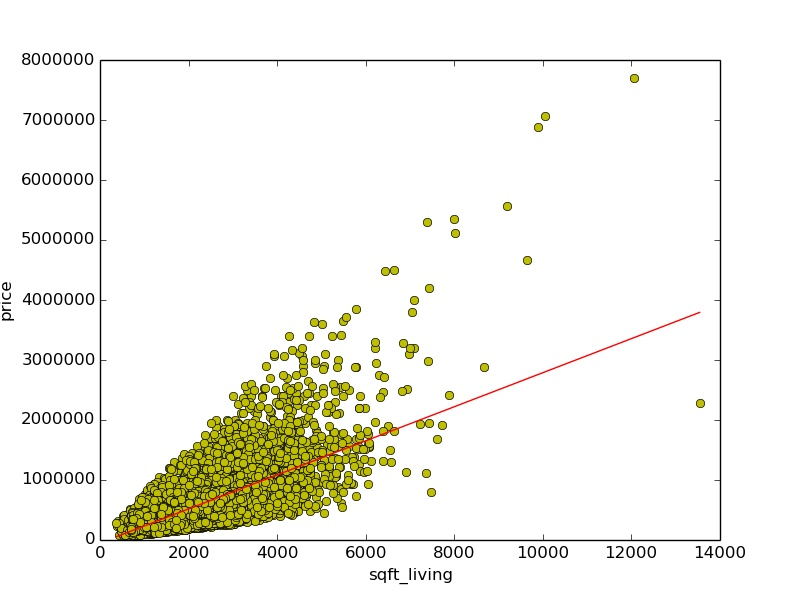
\includegraphics[width=0.5\textwidth]{../result/required_train_normal_equation.jpg}
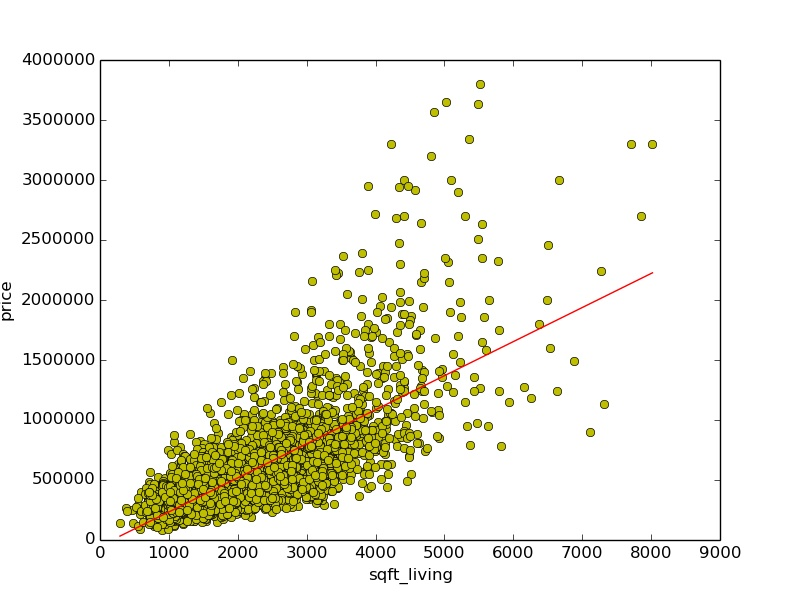
\includegraphics[width=0.5\textwidth]{../result/required_test_normal_equation.jpg}

The above scatter-plots show the results. Left one is training data and right one is test data. The fitting function is $$\mathbf{price}=283.842\times\mathbf{sqft\_living}-49800.406$$ and RMSE is 264054.500.

\section{Newton's Method}
Let $X$ and $y$ be the feature and label. Newton's method sets the original parameter $\theta_0$ manually and gets $$\theta_i=\theta_{i-1}-H^{-1}\nabla J(\theta).$$ Here $H=\nabla^2J(\theta)$ is the Hessian matrix. For linear regression, $$\nabla J(\theta)=X^TX\theta-X^Ty$$ and $$H=X^TX.$$

The Newton's method converges in 10 iterations. In fact, it will converge in one iteration. This is because $$\theta_1=\theta_0-H^{-1}\nabla J(\theta)= \theta_0-(X^TX)^{-1}(X^TX\theta-X^Ty)=(X^TX)^{-1}X^Ty.$$
Which is the same as normal equation.

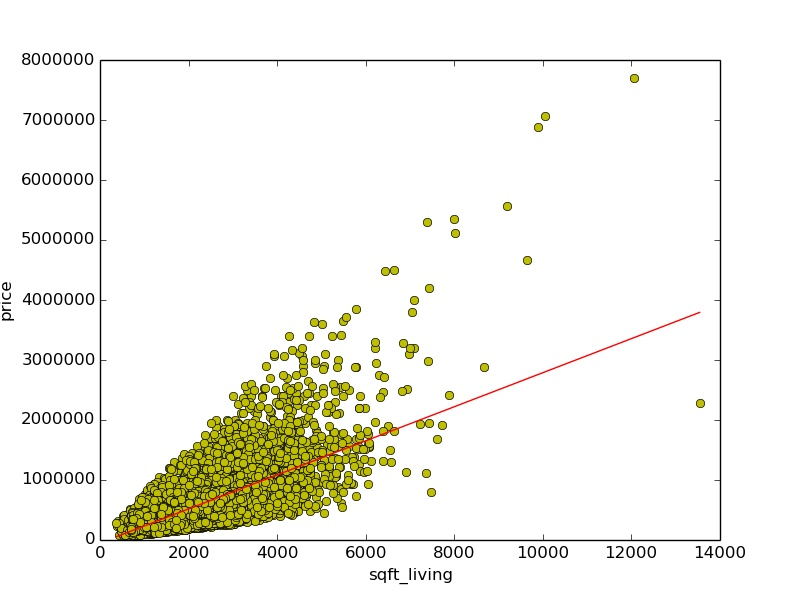
\includegraphics[width=0.5\textwidth]{../result/required_train_newtons_method.jpg}
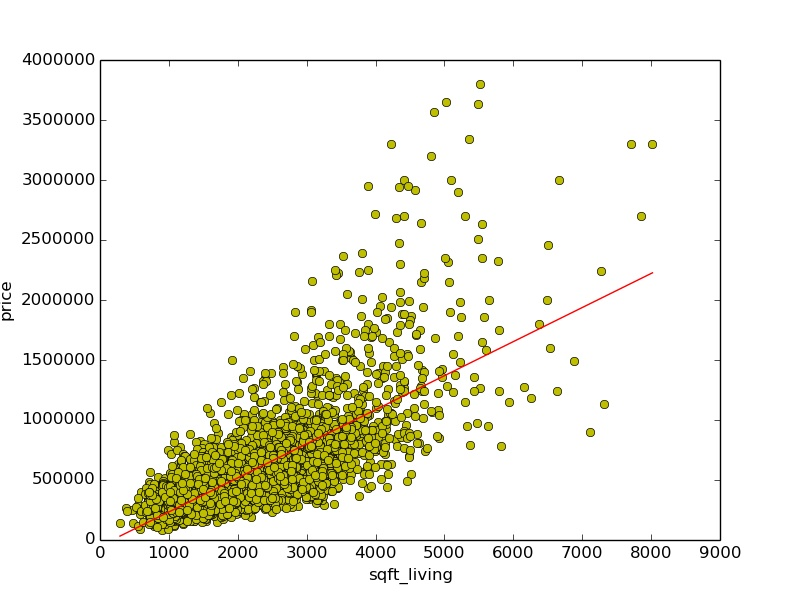
\includegraphics[width=0.5\textwidth]{../result/required_test_newtons_method.jpg}

The above scatter-plots show the results. Left one is training data and right one is test data. The fitting function is $$\mathbf{price}=283.842\times\mathbf{sqft\_living}-49800.406$$ and RMSE is 264054.500. The result is the same as normal equation.

\section{Gradient Descent}
Let $X$ and $y$ be the feature and label. Gradient Descent sets the original parameter $\theta_0$ manually and gets $$\theta_i=\theta_{i-1}-\alpha\nabla J(\theta).$$ Here $\alpha$ is the learning rate. For linear regression, $$\nabla J(\theta)=X^TX\theta-X^Ty.$$

We set $\alpha=0.1/n$ which $n$ is the number of samples. The gradient descent converges in 1000 iterations.

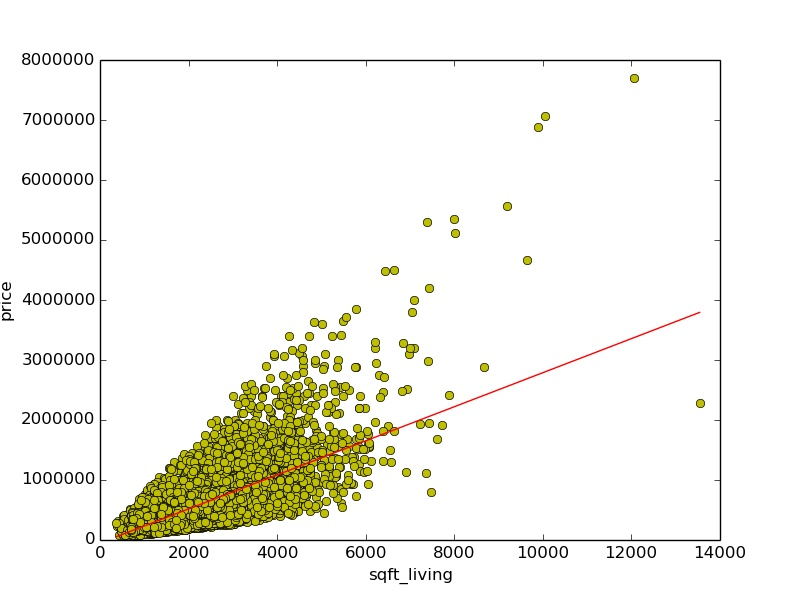
\includegraphics[width=0.5\textwidth]{../result/required_train_gradient_descent.jpg}
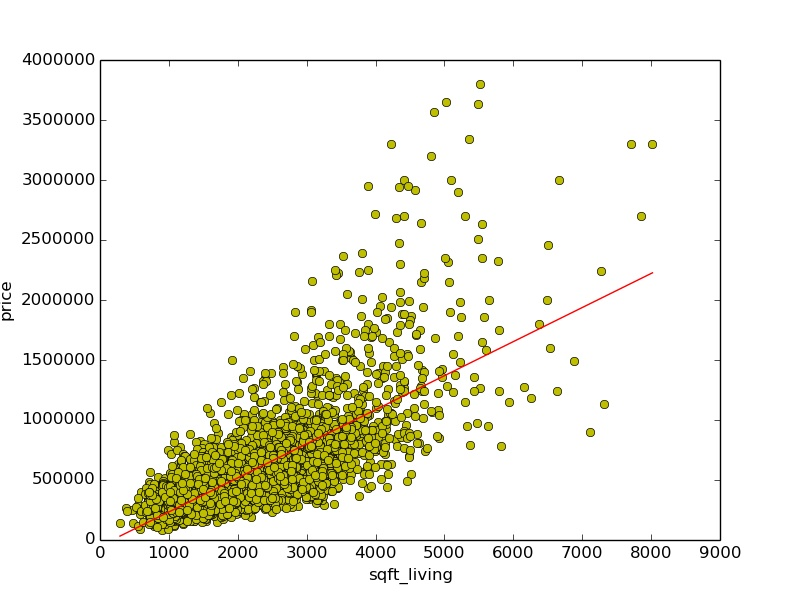
\includegraphics[width=0.5\textwidth]{../result/required_test_gradient_descent.jpg}

The above scatter-plots show the results. Left one is training data and right one is test data. The fitting function is $$\mathbf{price}=283.842\times\mathbf{sqft\_living}-49800.406$$ and RMSE is 264054.500. The result is the same as normal equation and Newton's method.

\section{Optional Task}
We use {\bf sqft\_living} and {\bf bedrooms} to predict {\bf price}. We use all the three methods and get the same results. The fitting function is $$\mathbf{price}=314.850\times\mathbf{sqft\_living} -53259.436\times\mathbf{bedrooms}+65820.347$$ and RMSE is 259160.225.

\end{document}